\section{Realisering og test}
\label{sec:research}

Kretsen i figur \ref{fig:kretsdiagram} ble realisert med komponentene i tabel \ref{tab:comp}.

\begin{table}[!tbp]
    \centering
    \caption{Komponenter brukt i differensialforsterkeren.}
    \label{tab:comp}
    \begin{tabular}{lll}
    Komponent  & type          & verdi                  \\ \hline
    Q$_1$      & 2N7000        &                        \\
    Q$_2$      & 2N7000        &                        \\
    Q$_3$      & VP2106        &                        \\
    Q$_4$      & VP2106        &                        \\
    Q$_5$      & 2N7000        &                        \\
    Q$_6$      & 2N7000        &                        \\
    R$_{P}$   & Potensiometer  & \text{10k$\Omega$}     \\
    R$_{P1}$  &                & \text{20k$\Omega$}     \\
    R$_{P2}$  &                & \text{10k$\Omega$}     \\
    R$_{S}$   &                & \text{1k$\Omega$} 
    \end{tabular}
    \end{table}

    \begin{figure}[!hbt]
        \centering
        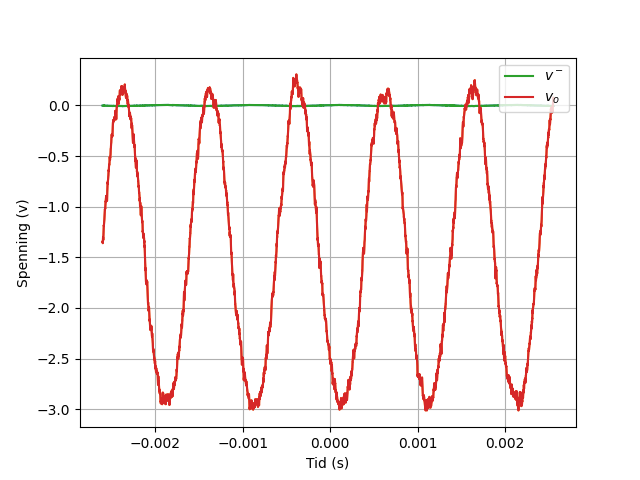
\includegraphics[scale=0.5]{./Images/03Research/åpenløkkeplain.png}
        \caption{Åpen-løkkeforsterkning med en inngangssignal på 5mV.}
        \label{fig:åpenløkke}
    \end{figure}

    Dette gav en forsterkning på $A \approx 350$ og en THD på $-27.6dB$ med en inngangssignal på 5mV og 1 KHz, det ble også observert lavere forsterkning og høyere THD ved høyere ingangssignal og når inngangssignalet gitt høyere enn 10mV så ble det observert klipping i utgangssgnalet som vist i figur \ref{fig:åpenløkke15mv}

    \begin{figure}[!hbt]
        \centering
        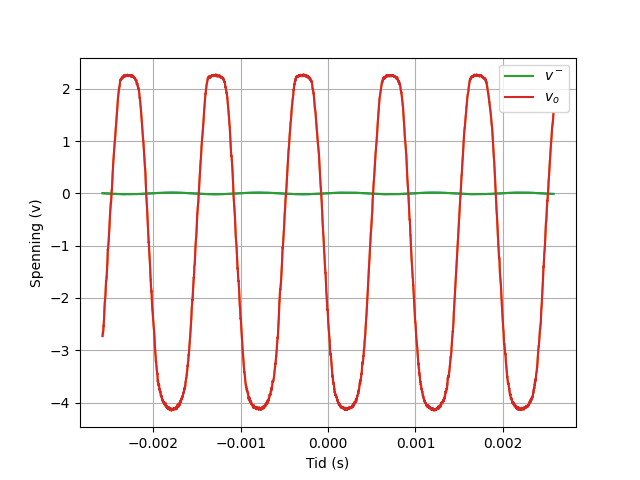
\includegraphics[width=.6\linewidth]{./Images/03Research/åpenløkkeplain15mv.png}
        \caption{Åpen-løkkeforsterkning med en inngangssignal på 15mV.}
        \label{fig:åpenløkke15mv}
    \end{figure}

Dette kan skyldes at det ikke er tilstrekkelig med spenningsforsyning $V^+$ og $V^-$ da tilsvarende klipping også forekom ved en inngangssignal på 5mV når spenningsforsyningen ble redussert.

Måling av THD og forsterkning $A$ ved sinuspåtrykk med frekvens f = 1 kHz med både 100 \text{$\Omega$} og 100 k\text{$\Omega$} er plottet inn i tabell \ref{tab:lastmotstand} utgangssignalene er vist i figur

\begin{table}[!hbt]
    \centering
    \caption{Forsterkning og THD ved ulik last motstand.}
    \label{tab:lastmotstand}
    \begin{tabular}{lll}
    $R_0$                & A   & THD[dBc]     \\ \hline
    0                    & 348 & -36.7        \\
    100 \text{$\Omega$}  & 91  & -7.7         \\
    100 \text{$K\Omega$} & 346 & -37.0       
    \end{tabular}
    \end{table}

    \begin{figure}[!hbt]
        \centering
        \begin{subfigure}{.5\textwidth}
            \centering
            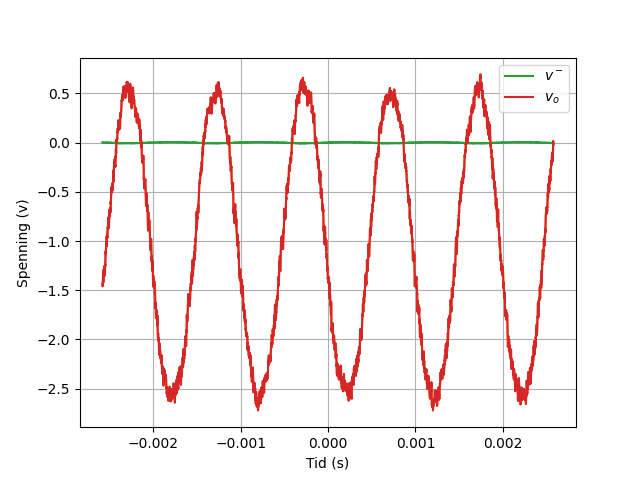
\includegraphics[width=1\linewidth]{./Images/03Research/åpenløkkeplain100kohm.png}
            \caption{Åpen-løkkeforsterkning med lastmotsand på 100 k\text{$\Omega$}}
            \label{fig:100k}
        \end{subfigure}%
        \begin{subfigure}{.5\textwidth}
            \centering
            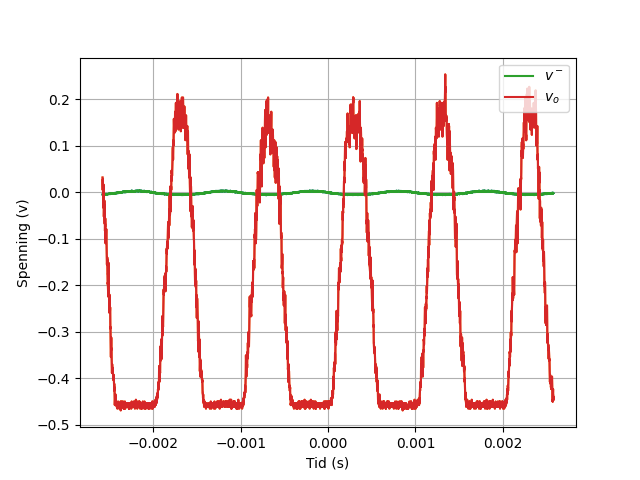
\includegraphics[width=1\linewidth]{./Images/03Research/åpenløkkeplain100ohm.png}
            \caption{Åpen-løkkeforsterkning med lastmotsand på 100 \text{$\Omega$}}
            \label{fig:100}
        \end{subfigure}
        % \caption{}
        % \label{fig:test}
    \end{figure}

    Siden spenningen blir lavere over lastmotstanden ved lav motstand kan det tenkes at utgangsmotstanden  til systemet har noe å si da det skjer et spenningsfall før lastmotstanden i motsetning til en høy lastmotsand da tilnermet alt spenningsfallet skjer over denne.

    \begin{figure}[!hbt]
        \centering
        \begin{subfigure}{.5\textwidth}
            \centering
            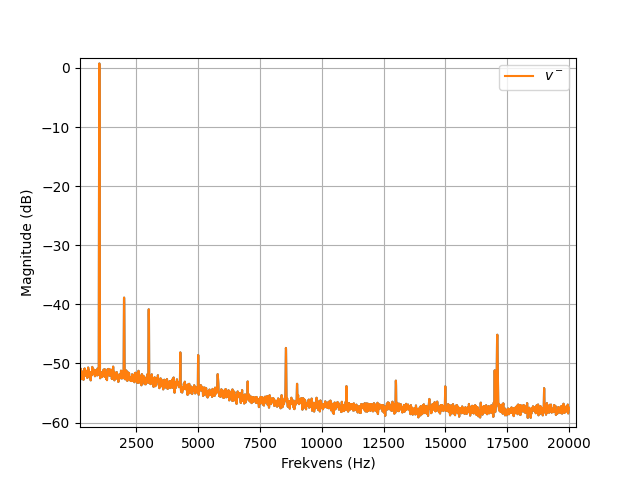
\includegraphics[width=1\linewidth]{./Images/03Research/spektrum100k.png}
            \caption{Åpen-løkkeforsterkning med lastmotsand på 100 k\text{$\Omega$}}
            \label{fig:100kspek}
        \end{subfigure}%
        \begin{subfigure}{.5\textwidth}
            \centering
            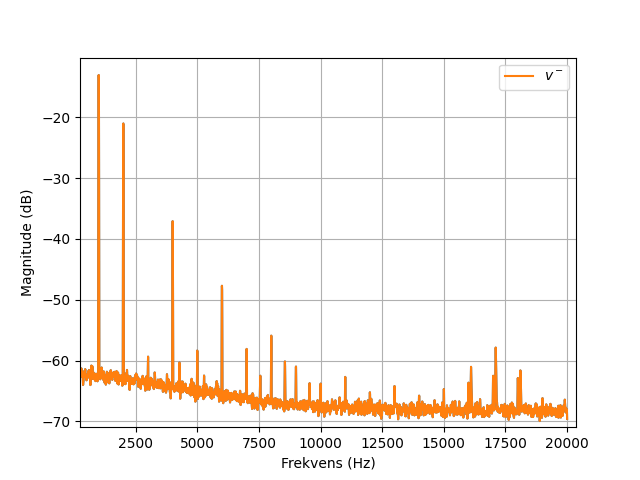
\includegraphics[width=1\linewidth]{./Images/03Research/spektrum100.png}
            \caption{Åpen-løkkeforsterkning med lastmotsand på 100 \text{$\Omega$}}
            \label{fig:100spek}
        \end{subfigure}
        \caption{Frkvensspekter for lastmotsand på 100 k\text{$\Omega$} og 100 \text{$\Omega$}}
        \label{fig:Frkvensspekter}
    \end{figure}

Det er observert at lav lastmotstand også gir mer overharmonisk støy i figur \ref{fig:Frkvensspekter}.

